\chapter{\xlabel{pol2_advanced}POL-2 -- Advanced Data Reduction}
\label{sec:advanced}


The \poltwomap\ tool for reducing POL-2 data was originally released for
general science community use several years ago. The fact that its
development remains ongoing directly reflects the continuing advances
made at the cutting edge of POL-2 data reduction and analysis.

This advanced section of the POL-2 data reduction documentation aims
to provide users with additional tools and options with which to refine their
individual POL-2 data reduction processes.

For further ideas, see \cref{Section}{sec:tailoredDR}{Tailoring a reduction}.

\section{\xlabel{addingdata}Adding new observations}

If a user receives additional data after an initial POL-2 reduction of a partial dataset,
then it is almost always easier (and the process more robust) for a user to simply
re-run the reduction process ''from scratch'' for the whole, augmented dataset.
Despite the associated additional processor time cost, therefore, users are generally
recommended to adopt this approach, rather than to attempt to combine new
observations with pre-existing \poltwomap\ reduction products.

For completeness, however, this section describes the six-step process of
combining data for one or more new POL-2 observations into existing $I$, $Q$,
and $U$ maps and vector catalogue created by an earlier run of \poltwomap.
\begin{enumerate}

\item Create a text file listing all the existing auto-masked $I$ maps
  for individual observations stored in the directory specified by
  Parameter \param{MAPDIR}, and then add in the raw data files for the new
  observations. The auto-masked $I$ maps have names that end in
  \file{$\_$imap.sdf}.

\begin{terminalv}
% ls maps/*imap.sdf > infiles.list
% ls rawdata/*.sdf  >> infiles.list
\end{terminalv}


\item Create a new auto-masked, co-added $I$ map including the new
  observation. The \xref{calcqu}{sun258}{CALCQU} and \makemap\ commands
  will be run on the new
  data and the resulting maps combined with the existing maps derived
  from the older observations to create the new map:

\begin{terminalv}
% pol2map in=^infiles iout=iauto_new qout=! uout=! mapdir=maps \
     qudir=qudata
\end{terminalv}


\item A decision needs to be taken as to whether to re-create all the
  externally masked maps using external masks defined by the new
  auto-masked map. This will be the case if the auto-masked map has
  been changed significantly by the addition of the new
  observation. To do this, it is necessary to compare the old and new
  masks. The old masks should have been created earlier using the
  \param{MASKOUT1} and \param{MASKOUT2} parameters (see Step~3 in
  \cref{Section}{sec:dr}{POL-2 Data Reduction -- The Theory}). To
  create the new masks that would be generated from the new
  auto-masked map, use this command:

\begin{terminalv}
% pol2map  in=^infiles iout=! qout=! uout=! mapdir=maps mask=iauto_new \
     maskout1=astmask_new  maskout2=pcamask_new
\end{terminalv}

\item Decide if the addition of the new data has changed the masks
  significantly. This involves comparing \file{astmask.sdf} and
  \file{astmask$\_$new.sdf} (and also \file{pcamask.sdf} and
  \file{pcamask$\_$new.sdf}).


\item If the mask has changed significantly and all observations need
  to be reprocessed using the new mask, or if \task{skyloop} is being used,
  remove the existing externally masked maps so that they will be re-created by
  the next invocation of \poltwomap.  Note that this will increase the length of
  time taken by Step~6 enormously.

  Ensure that the new auto-masked co-add is used in place of the old one, in order to
  define any new masks needed in future:

\begin{terminalv}
% rm mapdir/*Qmap.sdf mapdir/*Umap.sdf mapdir/*Imap.sdf
% mv iauto.sdf iauto_old.sdf
% mv iauto_new.sdf iauto.sdf
\end{terminalv}

\item Re-create the necessary externally masked maps and co-adds, and
  then create the new vector catalogue:

\begin{terminalv}
% pol2map in=qudata/\* iout=iext_new qout=! uout=! mapdir=maps \
     mask=iauto
% pol2map in=qudata/\* iout=! qout=qext_new uout=uext_new mapdir=maps \
     mask=iauto ipref=iext_new cat=mycat_new debias=yes
\end{terminalv}
\end{enumerate}


\section{\xlabel{pixelsize}Experimenting with pixel sizes}

Currently,the default map pixel size is 4\si{\arcsecond} at both
850 and \SI{450}{\micro\metre}. The pixel size is controlled by the
\param{PIXSIZE} parameter in the \smurf\ \poltwomap\ command:

\begin{terminalv}
% pol2map pixsize=12
\end{terminalv}


The following four-step example shows how to investigate the impact of
changing pixel size.  In this example, 12\si{\arcsecond}
pixels and 7\si{\arcsecond} pixels are compared.

\begin{enumerate}
\item Begin with an auto-masked total-intensity map from the raw
  data. For instance:

\begin{terminalv}
% pol2map in=^myfiles.list iout=iauto12 pixsize=12 qout=! uout=! \
     mapdir=maps12 qudir=qudata
\end{terminalv}


\item Create AST and PCA masks with 12\si{\arcsecond} pixels from the
  \file{iauto12.sdf} file:


\begin{terminalv}
% pol2map in=qudata/\* iout=! qout=! uout=! mapdir=maps12 mask=iauto12 \
     maskout1=astmask12 maskout2=pcamask12
\end{terminalv}

\item Create masks with 7\si{\arcsecond} pixels by resampling the
  12\si{\arcsecond} masks created at Step~2. This is done using the
  \Kappa\ \xref{\task{sqorst}}{sun95}{SQORST} command:

\begin{terminalv}
% sqorst  mode=pixelscale pixscale=\'7,7,7E-05\' in=astmask12 out=astmask7
% sqorst  mode=pixelscale pixscale=\'7,7,7E-05\' in=pcamask12 out=pcamask7
\end{terminalv}

\item Create the 7\si{\arcsecond} externally masked $I$, $Q$, and $U$ maps
  using the above 7\si{\arcsecond} masks (note the \texttt{mask}
  parameter value is enclosed in single \emph{and} double quotes).

\begin{terminalv}
% pol2map in=qudata/\* iout=iext7 qout=qext7 uout=uext7 masktype=mask \
                  mask="'astmask7,pcamask7'" mapdir=maps7 ipref=iext7  \
                  cat=cat7 debias=yes
\end{terminalv}
\end{enumerate}

\begin{tip}
  Using larger pixels usually produces slower convergence, and so the
  above process will take longer than usual---be patient!

  Using larger pixels can sometimes encourage smooth blobs and other
  artificial features to appear in the map. The \file{iauto12.sdf} file
  should be examined to check that it does not have such artificial
  features.

  Check the masks (\file{astmask12.sdf} and \file{pcamask12.sdf}) to make sure they
  look reasonable.

  It is usually advisable to leave \param{PIXSIZE} at its default value
  and instead use the \param{BINSIZE} parameter to control the bin size in
  the vector catalogue---see \cref{Section}{sec:pol2map-pixelsize}{Changing pixel size in pol2map}).
\end{tip}

\section{\xlabel{IPerror}Investigating systematic error in IP}


The error on the IP is reported to be of the order of 0.5\%.  It is
possible to investigate the effects of the systematic error in IP by
creating maps using the upper and lower limits on the IP value. The
\task{makemap} configuration parameter called \xparam{IPOFFSET}{ipoffset}
can be used to conduct such an investigation. To use it, run \poltwomap\ twice,
as follows:

\begin{terminalv}
% pol2map config="ipoffset=-0.25"
% pol2map config="ipoffset=0.25"
\end{terminalv}

This will produce maps using the upper and lower IP limits (a range of
0.5\%). If \poltwomap\ has already been run on POL-2 data, then a file will
already exist that was created using the mean IP (the mean IP is used
if \param{ipoffset} is omitted from the configuration value, or the
configuration parameter itself is omitted).

%\section{\xlabel{simulations}Simulated data}


\section{\label{sec:wcscopy}Adding WCS information back into a vector catalogue}
Vector catalogues produced by \poltwomap\ contain information about World Coordinate
Systems (WCS) in two different forms:

\begin{enumerate}
\item The catalogue contains ``RA'' and ``Dec'' columns that hold the sky position
(FK5, J2000) of each vector, in radians.
\item The catalogue header contains a Starlink ``WCS FrameSet'' which defines
(amongst other things) the projection from pixel coordinates within
the $I$, $Q$, and $U$ mosaics, to RA and Dec. This FrameSet is used by Starlink software, together
with the pixels coordinates stored in the ``X'' and ``Y'' columns, to determine
the RA and Dec of each vector. The WCS FrameSet also defines the polarimetric
reference direction used by the $Q$, $U$, and ANG values. See
``\xref{Using World Co-ordinate Systems}{sun95}{se_wcsuse}''
within \xref{SUN/95}{sun95}{} (the \KAPPA\ manual) for more information on
the ways in which Starlink software handles WCS information.
\end{enumerate}

Starlink software such as \polpack, \Kappa, and \gaia\ rely on the WCS
FrameSet for all WCS-related operations (drawing annotated axes, aligning
data sets, \emph{etc}). Thus, problems are likely to arise if the WCS FrameSet
is removed from the vector catalogue. This could happen if (for instance)
inappropriate software is used to process an existing catalogue, creating a
new output catalogue. Under such circumstances, the WCS FrameSet might
not be copied to the output catalogue, causing subsequent WCS-related
operations to fail. It is safe to use \POLPACK, \KAPPA, \GAIA\ and
\xref{\textsc{Cursa}}{sun190}{}), as all these packages copy the WCS
FrameSet to any new output catalogues. Unfortunately, the popular
\topcat\ catalogue browser (see
\url{http://www.starlink.ac.uk/topcat/}) and the STILTS package
(\url{http://www.starlink.ac.uk/stilts/}) upon which it is based, do
\emph{not} copy the WCS FrameSet to any output catalogues.

For this reason, \POLPACK\ contains a command that can be used to copy the
WCS FrameSet from one catalogue to another.  For example: a user creates
the catalogue \file{mycat.FIT} using \poltwomap, uses \textsc{Topcat}
to remove low signal-to-noise vectors, an then saves the results to a new catalogue
called \file{selcat.FIT}. The WCS FrameSet would then be missing from \file{selcat.FIT},
and so it would be necessary to copy it back into place again from the original catalogue
file, \file{mycat.FIT}. To do this, the ``\xref{polwcscopy}{sun223}{POLWCSCOPY}''
command can be used:

\begin{terminalv}
% polwcscopy in=selcat ref=mycat out=selcat2
\end{terminalv}

This would create a third catalogue \file{selcat2.FIT}, which would be a copy of
\file{selcat.FIT}, but with the WCS information inherited from \file{mycat.FIT}.


\section{\xlabel{vectorerrorremodelling}Re-modelling the error estimates in a POL-2 vector catalogue}

If the \texttt{MAPVAR=YES} option is used when running the \smurf\ \poltwomap\ script, the I, Q and U error estimates in the resulting vector catalogue will be based on the spread of pixel values at each point on the sky in the I, Q and U maps made from individual observations. Thus, if 20 observations are processed by \poltwomap\ to create a vector catalogue, then each I, Q or U error estimate in the vector catalogue will be based on the spread of 20 independent measurements of I, Q or U.  Even though 20 observations is a lot of POL-2 data, 20 is still a fairly small number from which to produce an accurate estimate of the error. Consequently, it is usual to see a large level of random ``noise'' on the error estimates, as in the following example, which shows the total intensity (I) error estimates taken from a 12\si{\arcsecond} vector catalogue near Ophiuchus L 1688 (\cref{Figure}{fig:originalerrors}{}).

\begin{figure}[ht!]
\begin{center}
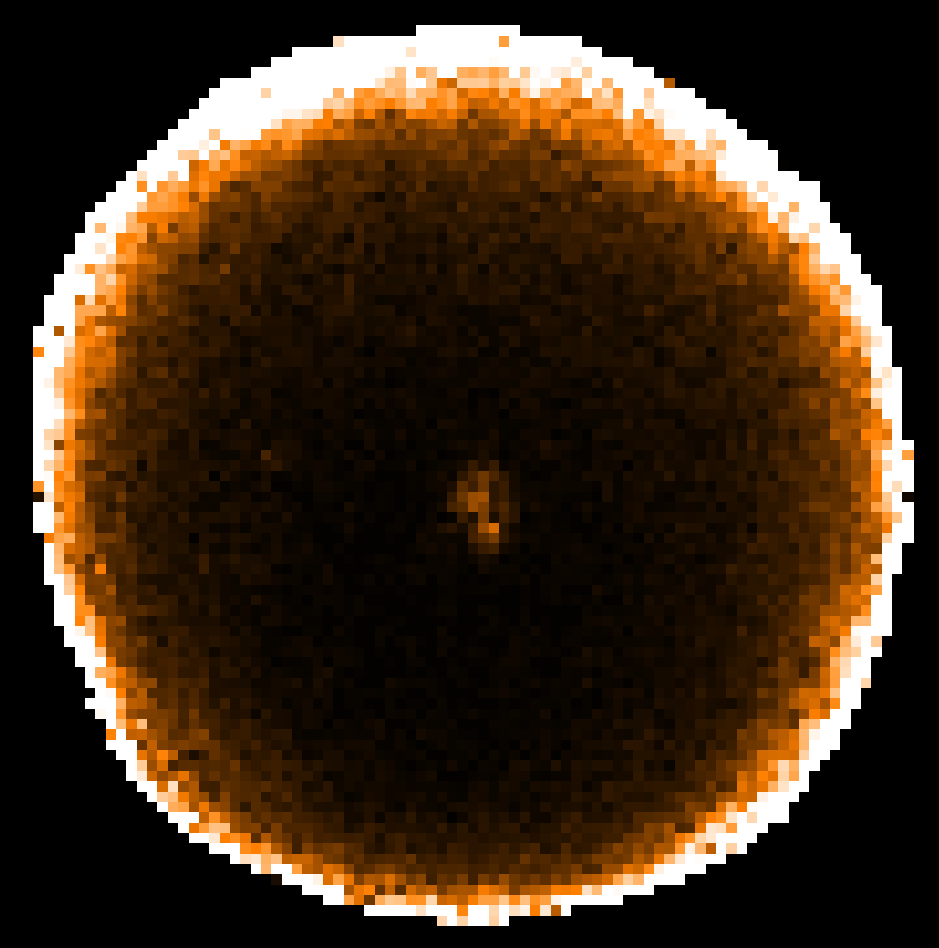
\includegraphics[width=0.46\linewidth]{sc22-ophl1688-noise_on_error-1.png}
\caption [Original Error Estimates in POL-2 Vector Catalogue for Oph L1688]{
  The initial total intensity (I) error estimates taken from a 12\si{\arcsecond} vector catalogue near Ophiuchus L 1688. Note that the noise level increases towards the edge of the map due to there being fewer bolometer samples per pixel near the edge.
\label{fig:originalerrors}
}
\end{center}
\end{figure}

The uncertainty on the error estimate can cause some vectors that are clearly wrong (e.g. because they are very different from nearby vectors) to have anomalously low error estimates and so to be included in the set of ``good'' vectors (i.e. vectors that pass some suitable selection criterion based on the noise estimates).

One simple solution to this could be to apply some spatial smoothing to the error estimates. This would be a reasonable thing to do if there were no compact sources in the map. The errors close to a compact source are generally higher than those in a background region because of factors such as pointing errors, calibration errors, etc. These factors cause a compact source to appear slightly different in each observation, and so cause higher error estimates in the vector catalogue. The above error estimates map shows this effect in the higher values at the very centre. Simply smoothing this map would spread that central feature out, artificially decreasing the peak error and increasing the errors in the neighbouring background pixels.

An alternative to smoothing is to split the total noise up into several different components, create a model of each component , and then add the models together. The \task{pol2noise} script in \smurf\ enables the user to re-model the noise estimates in a vector catalogue using such an approach. This facility is used by setting \texttt{MODE=REMODEL} on the \task{pol2noise} command line:

\begin{terminalv}
% pol2noise mycat.FIT mode=remodel out=newcat.FIT exptime=iext debiastype=mas
\end{terminalv}


This  creates an output catalogue (\file{newcat.FIT}) holding a copy of the input catalogue (\file{mycat.FIT}), and then calculates new values for all the error columns in the output catalogue. The new I, Q and U error values are first derived from a three component model of the noise in each quantity, and then errors for the derived quantities (PI, P and ANG) are found. New values of PI and P are also found using the specified de-biasing algorithm. The file \file{iext.sdf} holds the total intensity coadd map created by \poltwomap\ and is used to define the total exposure time in each pixel. The re-modelled total intensity error estimates are shown in (\cref{Figure}{fig:newerrors}{}).

\begin{figure}[ht!]
\begin{center}
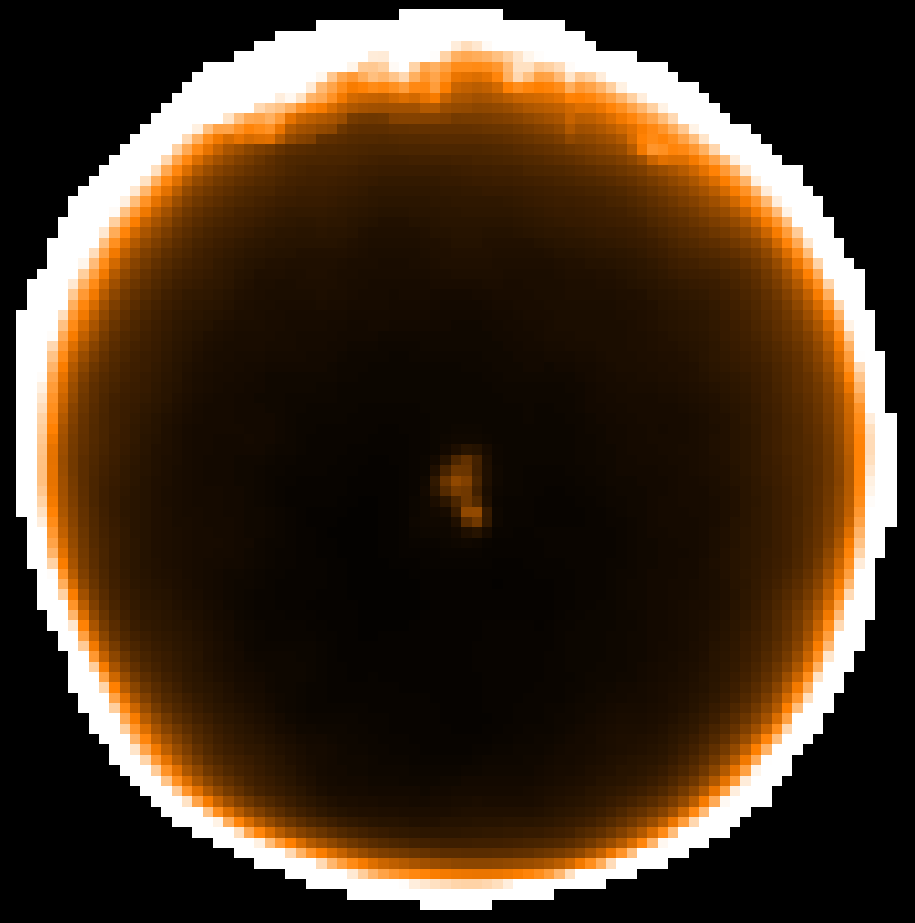
\includegraphics[width=0.46\linewidth]{sc22-ophl1688-pol2-noise-remod-1.png}
\caption [Remodelled Error Estimates in POL-2 Vector Catalogue for Oph L1688]{
  The re-modelled total intensity (I) error estimates taken from a 12\si{\arcsecond} vector catalogue near Ophiuchus L 1688. Note the reduced noise in comparison to \cref{Figure}{fig:originalerrors}{}.
\label{fig:newerrors}
}
\end{center}
\end{figure}

Most of the noise has gone without reducing the resolution. The script displays the original and re-modelled error estimates for each Stokes parameter (I, Q and U), the residuals between the two and a scatter plot (\cref{Figure}{fig:remodellingwindow}{}). The best-fitting straight lines through each scatter plot are also displayed.

\begin{figure}[ht!]
\begin{center}
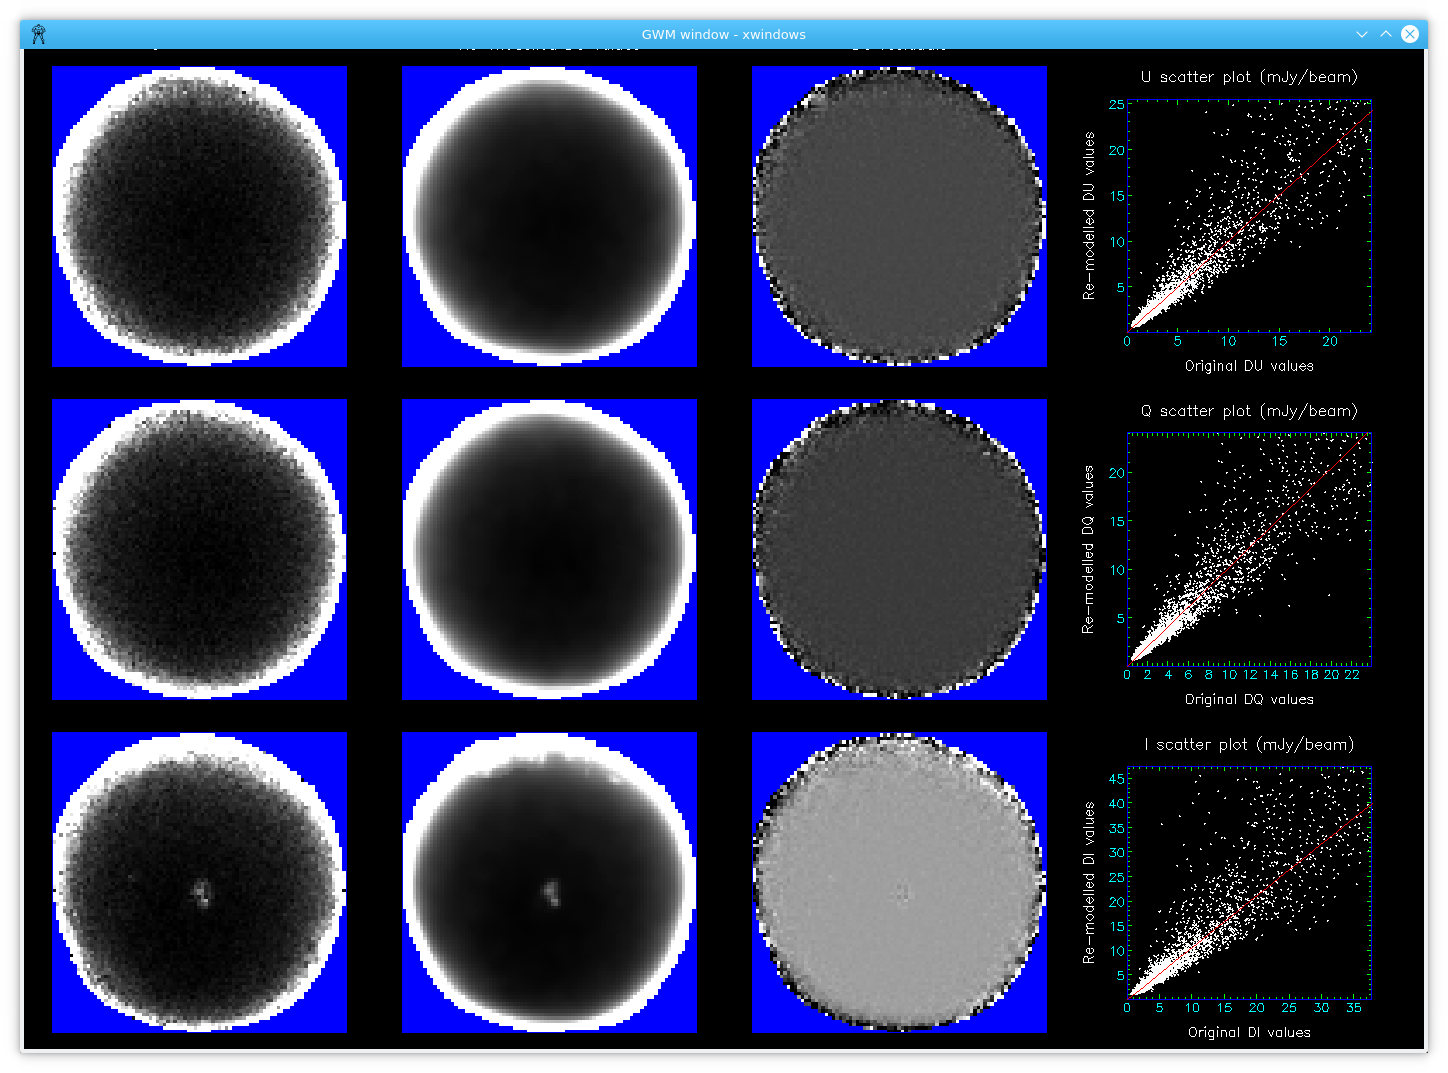
\includegraphics[width=0.46\linewidth]{sc22-ophl1688-pol2noise-fitting-1.png}
\caption [Plotting Window produced During POL-2 Vector Catalogue Error Estimate Remodelling for Oph L1688]{Example of the output displayed during the POL-2
vector catalogue error estimate re-modelling process. Comparison Stokes parameter
(I, Q and U) plots are shown, together with residuals images and associated straight line fits.
}
\label{fig:remodellingwindow}
\end{center}
\end{figure}

The three components used to model the error on each Stokes parameter (I, Q or U) are described below:

\begin{enumerate}
\item {\bf The background component:} This is derived from an exposure time map  (obtained from
iext.sdf in the above example). The background component is equal to $A.tB$, where $t$ is 
the exposure time at each pixel and $A$ and $B$ are constants determined by doing a linear fit 
between
the log of the noise estimate in the catalogue (DQ, DU or DI) and the log of the exposure time
(in practice, $B$ is usually close to -0.5). The fit excludes bright source areas, but also excludes a
thin rim around the edge of the map where the original noise estimates are subject to large
inaccuracies. Since the exposure time map is usually very much smoother than the original
noise estimates, the background component is also much smoother.
\item {\bf The source component:} This represents the extra noise found in and around compact sources caused by pointing errors, calibration errors, etc. The background component is first subtracted from the catalogue noise estimates and the residual noise values are then modelled using a collection of Gaussians. This modeling is done using the \texttt{GaussClumps} algorithm provided by the \task{findclumps} command in the Starlink \cupid\ package. The noise residuals are first divided into a number of ?islands?, each island being a collection of contiguous pixels with  noise residual significantly higher than zero (this is done using the \texttt{FellWalker} algorithm in \cupid). The \texttt{GaussClumps} algorithm is then used to model the noise residuals in each island. The resulting model is smoothed lightly using a Gaussian kernel of FWHM 1.2 pixels.
\item {\bf The residual component:} This represents any noise not accounted for by the other two models. The noise residuals are first found by subtracting the other two components from the original catalogue noise estimates. Any strong outlier values are removed and the results are smoothed more heavily using a Gaussian kernel of FWHM 4 pixels.
\end{enumerate}

The final model is the sum of the above three components. The new DI, DQ and DU values are found independently using the above method. The errors for the derived quantities (DPI, DP and DANG) are then found from DQ, DU and DI using the usual error propagation formulae. Finally new P and PI values are found using a specified form of de-biasing (controlled by the parameter \texttt{DEBIASTYPE}).



\section{\xlabel{vectoredebiaschanging}Changing the de-biasing in a POL-2 vector catalogue}

The new \task{poledit} command in the Starlink \POLPACK\ package has an option to recalculate the PI (polarised intensity) and P (percentage polarisation) values using a specified form of de-biasing. If the existing catalogue is in file \file{mycat.FIT}, this can be done with:

\begin{terminalv}
% polpack
% poledit mycat newcat mode=debias debiastype=mas
\end{terminalv}

This will create a new file, \file{newcat.FIT}, containing a copy of \file{mycat.FIT}, but with new P and PI columns re-calculated from the existing Q, U, I and DPI values using the ?Modified Asymptotic? (MAS) bias estimator (any de-biasing used to create the original catalogue is ignored). The options for the \param{DEBIASTYPE} parameter are:

\begin{enumerate}
\item {\bf MAS:} De-bias using the modified asymptotic estimator;
\item {\bf AS:} De-bias using the asymptotic estimator;
\item {\bf None:} Do not include any de-biasing.
\end{enumerate}

\cref{Figure}{fig:poleditdebias-1}{} shows the results of using the \task{poledit} command with the various  \param{DEBIASTYPE} parameter options listed above.

\begin{figure}[ht!]
\begin{center}
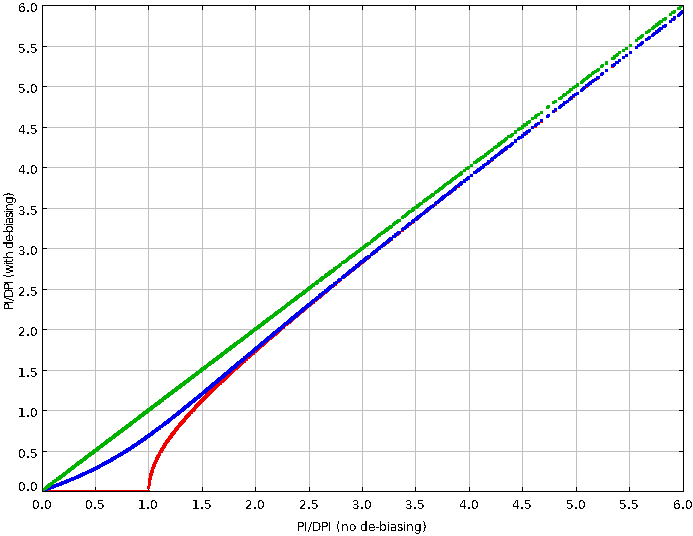
\includegraphics[width=0.46\linewidth]{sc22-poledit-debias.png}
\caption [The effects of using the various \task{poledit} debias options]{
  The effects of using the various \task{poledit} debias options. The horizontal axis is PI/DPI (polarised intensity signal to noise ratio) with no de-biasing. The vertical axis is the new PI/DPI value created with each of the \param{DEBIASTYPE} options listed above (red is ``AS'', blue is ``MAS'' and green is ``None'')
\label{fig:poleditdebias-1}
}
\end{center}
\end{figure}
